\section{重修线性代数8——分解 }
矩阵的分解,实际上是通过坐标变换来揭示矩阵所表示的线性算子性质。

在过去,人们靠公式的推导来简化计算,线性代数主要用在理论分析和解方程,其重点是表达线性变换的特征,在不同坐标上矩阵表示的相似性和标准形式。在计算机时代,人们关心矩阵的线性运算特征,抽取矩阵的线性放大特性和近似,应用于海量的数据存储和计算。代表着线性算子的一般矩阵的分解,特别是SVD分解,便成为今日关注的重点。

\subsection{满秩方阵的分解}
满秩的方阵对应着一个坐标变换,它可以分解为几个初等变换的乘积。这个分解的目的,在于计算上通过这些初等变换的操作,来解方程和求逆。

我们知道,对线性方程组,调换组中方程的次序,在方程的两边同乘以非零的数,以及将一个方程乘数,两边同加在另一个方程上,都不改变方程组的解。

从线性空间角度来看,这不过是在值域空间做坐标变换。方程的解x是b在矩阵列向量的线性组合系数,改变了这些向量的坐标表示,当然不改变b与矩阵列向量的线性表示关系。

我们把上面三种对方程组的操作称为初等变换,即:(1)两行(列)互换:$ \bm{R}_{i} \leftrightarrow \bm{R}_{j} $,(2)把某行(列)乘以一非零常数:$ k\bm{R}_{i}\rightarrow \bm{R}_{i} $ , 其中$ k\neq0 $,(3)把第i行(列)加上第j行(列)的k倍:$ \bm{R}_{i} + k\bm{R}_{j}\rightarrow \bm{R}_{i} $。初等矩阵即是将上述3种初等变换作用到单位矩阵的结果,分别记为  $ P_{ij},D_{i}(k),T_{ij}(k) $,对应于旋翻、缩放($ k=-1 $为翻转)和剪切的变换。初等变换对应于一个坐标变换,初等矩阵左乘矩阵A,则是对A行的变换,它相应于算子A的值域空间中的坐标变换。初等矩阵右乘矩阵A,则是对A进行列的变换,它相应于在算子A的定义域空间中坐标变换。

读者不难在头脑中想象到初等变换的矩阵形式,初等矩阵都是满秩的线性变换。从变换的含义马上得出它们的逆矩阵分别是$ P_{ij},D_{i}(1/k),T_{ij}(-k) $。

参考一下解方程中的高斯消去法,对于一个方阵A,它可以一系列行的初等变换,把它变成上三角阵$ U $,即$ P_{1}P_{2}\cdots P_{s}A=U $,因为这些是初等矩阵,很容易写出逆来相乘$ P_{s}^{-1}\cdots P_{2}^{-1}P_{1}^{-1}=L $,显然$ A = LU $. 消去法没有换行时,P都是下三角阵,则L是一个对角线都是1的下三角阵,这便是\textbf{LU分解}。三角阵的线性方程可以用迭代法求解,这个分解用来解方程和求行列式。

不难想象k秩的矩阵A,可以等价于对角线上左上角开始有k个1,其余都是0的矩阵。如果A是一个满秩的矩阵,它等价于单位矩阵。

对于n阶满秩方阵A求逆的计算,因为A的逆是一系列把它变成单位矩阵I的初等矩阵的乘积,把n阶单位矩阵拼在A的右边成为$ n\times 2 n$的增广矩阵$ (A\ I)$,然后对它进行初等行变换,直至左边的$ n\times n $那块是单位矩阵,右边那$ n\times n $部分就是A的逆。这个计算过程相当于$ A^{-1}(A\ I)=(I\ A-1) $。

\subsection{正交变换}

一般线性空间中坐标变换,在欧几里德空间里,包含着坐标的拉伸、旋转、翻转、剪切等变换,坐标轴之间可能是倾斜。这对只关心加法和数乘代数性质的线性空间,并没有什么关系。因为这抽象线性空间,根本没有“拉伸”和“倾斜”等几何的概念。长度和角度概念由内积运算定义的,要讲究这些,必须在内积空间里来谈论。

保持内积不变的坐标变换,也就是向量的长度和夹角,在不同坐标系上的表示都保持不变。这种坐标变换称为正交变换,物理上称么正变换。它的矩阵在实数域是正交阵,在复数域是酉阵。这直接可以从对偶算子和内积等式推出$ \langle y, \bar{x}\rangle=\langle Uy, Ux\rangle=\langle y,U^{*} Ux\rangle \rightarrow U^{*}U=I $,在实数域$ U^{*} = U^{T}  $. 以后我们都只在实数域上讨论,对于复数域,将转置换成共轭转置就行。

内积空间坐标表示必须在标准正交基上,这样才能保证同构关系。正交变换是把这各向同性直角坐标系,刚性地整体旋转和翻转,所以表示的向量长度和夹角在变换后保持不变。

对于线性变换的方阵,坐标变换是同样作用在算子的输入和输出空间,因为在内积空间上坐标变换必须是正交变换,在线性空间上相似的矩阵,在内积空间上未必做得到。例如非对称的矩阵有可能与一个对角阵相似,但未必有正交的坐标变换做到这一点。在内积空间(通过正交变换)与对角阵相似,当且仅当它是正规矩阵,正规矩阵A有$ A^{*}A  = AA^{*} $. 实数域上的对称阵和复数域上的厄米矩阵都是正规矩阵。

对于$ m\times n $矩阵A, $ m\ge n $可以分解成列向量的$ m\times n $单位正交集Q与一个$ n\times n $的上三角阵R相乘, $ A=QR $,这叫做\textbf{QR分解}。这个分解可以看作依次按照Gram-Schmidt方法对A中的列向量做正交化,Q就是单位正交化后的列向量,R中的元素是正交化过程中的内积。矩阵Q表现旋转和翻转部分的映射,R体现了缩放和剪切的畸变。

怎么把线性无关的列向量变成单位正交的向量组?这在几何上很直观。取矩阵A的第一个列向量$ A_1 $把它标准化(归一化) $ e_1 = A_1/\|A_1\| $ ,其中的长度放在R阵的第一个对角线元素上 $ R_{11}=\|A_1\| $,再取第二个列向量$  A_2  $,减去它在$ e_1 $的投影的向量$ x_2 = A_2 - \langle A_2, e_1 \rangle e_1 $,令 $ R_{12}=\langle A_2, e_1 \rangle $,再把它标准化$ e_2 = x_2/\|x_2\| ,\;\;R_{22}=\|x_2\|,\;\;e_1, e_2 $ 便是两个标准正交的向量。已经有了k-1个标准正交向量,取第k个列向量$ A_k $,减去它在这些标准正交向量的投影向量 $ x_{k} = A_{k} - \sum_{i=1}^{k-1} \langle A_{k}, e_i \rangle e_i $ ,将这些投影分别放在R阵中 $ R_{ki}= \langle A_k, e_i \rangle $ ,再把它标准化$ e_k = x_k/\|x_k\|, \; R_{kk}= \|x_k\| $,如此下去。这个过程叫做Gram-Schmidt正交化。显然,标准正交的向量构成Q矩阵 $ (e_1, e_2,\cdots ,e_n)=Q $,R是一个上三角阵,A=QR。对于矩阵的列向量不是线性无关时,Q阵略去0向量,最后添上与前面正交的标准向量。

在MATLAB和Octave中,用qr函数来计算行QR分解,指令为:[Q,R]=qr(A),分解为m*m的Q阵和m*n的R阵。

\subsection{线性算子对核与像空间的分解}

前面介绍过,表示线性算子的矩阵A,它的核Ker(A)是所有映射成零的向量集合,构成了X中的一个子空间;它的像Im(A)是所有映射得到向量的集合,构成了Y中的一个子空间。我们有线性代数的基本定理,表示为下图。

% TODO: \usepackage{graphicx} required
\begin{figure}[h]
	\centering
	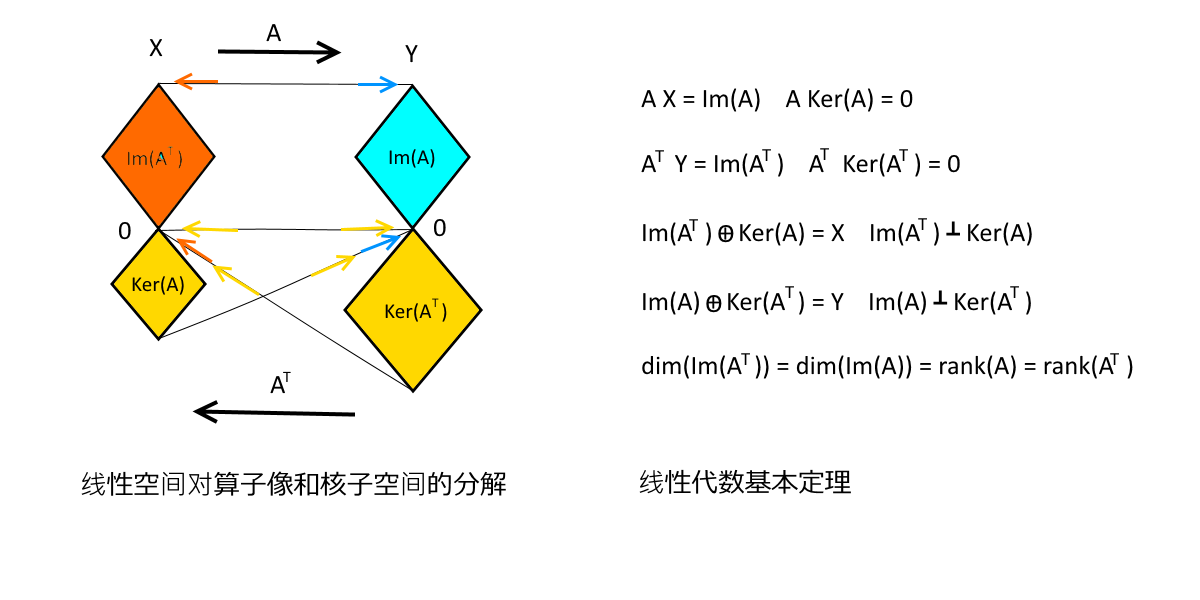
\includegraphics[width=0.7\linewidth]{pic/1604494yzy1do1yro41gva.png}
	\caption[代数学基本定理]{线性空间对算子像和核空间的分解}
	\label{fig:1604494yzy1do1yro41gva}
\end{figure}


算子A将输入空间X和输出空间Y,分别分解为正交的两个子空间的直和。

\[ Im(A^T)\oplus Ker(A)=X   Im(A)\oplus Ker(A^T)=Y"  \]%width="501" height="20" style="width: 501px; height: 20px;

X的线性子空间$ Im(A^T) $和Y的$ Im(A) $有相同的维数k,说明$ Im(A^T) $的基向量在算子映射下的像可以作为$ Im(A) $的基向量,算子A局限这子空间中,在这两个基的矩阵表示是k阶单位向量。

在$ Im(A^T) $子空间选取k个线性无关的向量 $ {V_1,V_2, \cdots,V_k} $,在Ker(A) 选取n-k个 $ {V_{k+1}, \cdots,V_n} $,共同构成X的一个基。令$ U_i= AV_i, i=1, 2, \cdots,k $,它们构成子空间Im(A)的基,在Ker(AT) 选取m-k个$  {U_{k+1}, \cdots,U_n} $,共同构成Y的一个基。在这两个空间的基上,线性算子$ \alpha $表示表示为主对角线上前r个是1,其他全是0的“k秩准单位阵”D。

\[U^{-1}AV = \begin{pmatrix}I_k&0\\0&0\end{pmatrix}\]

秩数为k的线性算子在合适的基上都可以表示为“k秩准单位阵”,即k秩的矩阵A可以分解成 $ A = UDV^{-1} $,D是与A的行列数秩数相同的“准单位阵”,V和U分别是X和Y空间里新旧坐标的变换矩阵。注意到构造V和U时基时,除了要求前k个$ U_i = AV_i $,外,其他的基向量是在指定的子空间内,任意选取线性无关的即可,所以除了D是由矩阵的秩唯一确定之外,有无数个不同U和V的分解。

\subsection{奇异值分解}

线性算子对核和像空间的分解只是简单地区分对算子的映射值“有影响”和“无影响”的两部分。许多的应用希望了解线性算子作用在不同方向的放大特性,这涉及到向量的长度和方向,必须在内积空间中考虑,它要求坐标变换不改变列向量表示的长度和夹角,即坐标变换必须是正交变换。

线性算子A把输入空间X分解成正交的$ Im(A^T) $子空间和零空间$ Ker(A) $的直和,A把零空间中向量都映成了零向量,$ Im(A^T) $子空间中的向量与A像空间$ Im(A) $的向量一一对应。所以对算子放大特性的研究,只需要考虑它对$ Im(A^T) $子空间中向量的作用。想象一下线性算子A作用在$ Im(A^T) $子空间中一个单位向量v,v沿着各种可能的方向转动,它的像Av的长度和方向也随之变化,选取能够让它的像有最大长度$ \sigma_1 $的v,记为$ V_1 $,这个像的单位向量记为$ U_1 $,有$ AV_1=\sigma_1U_1 $;然后在$ Im(A^T) $中与$ V_1 $正交的子空间里,再次选取具有最大长度$ \sigma_2 $像的$ V_2 $;如此可以进行k次,得到k个正交单位向量$ {V_1,V_2,\cdots,V_k} $,它们是一组$ Im(A^T) $中标准正交基,有$ AV_i =\sigma_iU_i,,i=1, 2, \cdots,k $,放大率$ σ_i $逐次减小,这便是线性算子A的放大特性。X空间中所有的向量可以分解成$ Im(A^T) $和$ Ker(A) $子空间中向量之和,后者被A映射为零向量。在零空间$ Ker(A) $里补足n-k个单位正交向量$ {V_{K+1},V_{K+2}, \cdots,V_n} $,以它们为基,A在上面的放大率为0,线性算子A在不同方向的放大率便直接反映在原空间坐标轴与对应像空间的坐标轴方向上。这些单位正交向量构成正交阵V,只要证明$ U_i $构成的矩阵U也是正交阵,就可以把它们看成是内积空间里的坐标变换,我们便能从奇异值分解中,得到线性算子对内积空间不同方向的放大特性。


% TODO: \usepackage{graphicx} required
\begin{figure}[h]
	\centering
	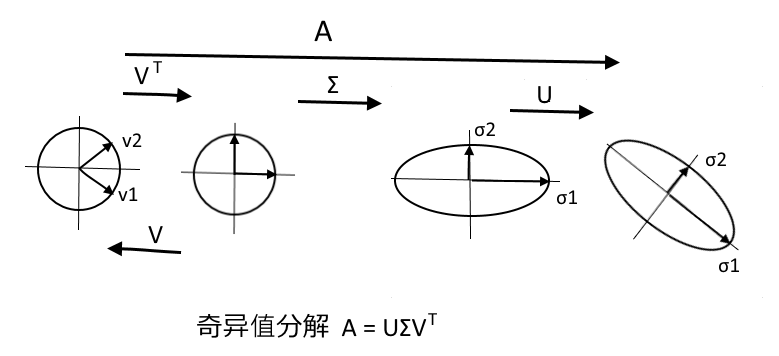
\includegraphics[width=0.7\linewidth]{pic/20450596leeoio001j6199.png}
	\caption{奇异值分解}
	\label{fig:20450596leeoio001j6199}
\end{figure}

\kaishu

奇异值分解(简称SVD)说:对于秩数为r的m*n矩阵A,可以分解成 $ A = U\sum V^T $,这里U是m阶正交阵,V是n阶正交阵,Σ是主对角线上是从大到小的正数$ \sigma_1,\sigma_2, \cdots , \sigma_k $,其余都是0的m*n矩阵。这些正数称为矩阵A的奇异值。

\songti

正交阵V表示一个只包含旋转和翻转的坐标变换,它的列向量表示在X空间中那个相互正交的新坐标轴单位向量。奇异值分解表达出A在这新坐标轴方向上,依次表现出从最大σ1到最小σk的向量长度放大率,直至退化到0的算子作用。U表示在Y空间经过正交变换的新坐标系统,它的前k个列向量作为新坐标轴的单位向量,依此对应着那些经过放大作用后的向量方向。矩阵Σ表达算子这些从最大到最小放大率和秩。

从上述$ AV_i=\sigma_iU_i $关系和正交阵V构造,在$ Ker(A^T) $中选取一组基向量补足列向量,让U矩阵满秩,我们知道不论U是什么都有分解式$ A = U\sum V^T $成立。现在证明U可以是正交阵。$ AA^T = (U\sum V^T)(V\sum^TU^T)  =  U(\sum\sum^T)U^T $,$ AA^T $是对称阵,它可以通过正交变换对角化,而$ \sum\sum^T $是对角阵,其对角线上的元素集合即特征值是由$ AA^T $唯一确定的,这意味着这里的U是那个特征向量组成的正交阵。

如何简单地计算V和放大系数$ \sigma_i $依上面相同的思路,注意到$ (A^TA) $是个半正定的对称方阵,它可对角化,有非负特征根在对角线上。通过解$ (A^TA) $的特征方程,求出特征根和单位特征向量,调整这些单位特征向量在矩阵中排列的顺序,使得对应的特征值从大到小,构造正交阵V,算子的放大系数便是这些特征根的正平方根。细节如下。

记$ Im(A^T) $里的向量$  {V_1,V_2, \cdots,V_k}  $与$ Ker(A)  $里 $ {V_{k+1}, \cdots, V_{n}} $,组成单位正交阵V,设$ AV_i=\sigma_iU_i , i=1, 2, \cdot,k,\sigma_i$是个正数$ ,AV_i=0,i=k+1, \cdots, n $,因为U的列向量也都是单位正交的,所以 有$  V^{-1}(A^TA)  =  (AV)^T(AV)$  $= $  $ U^Tdiag($  $\sigma_1^2,\sigma_2^2, \cdots, \sigma_r^2,0, \cdots,0)U = $   $ diag(\sigma_1^2,\sigma_2^2, \cdots, \sigma_r^2,0, \cdots,0) $,这式子表示正交的坐标变换V,把对称阵$ (A^TA) $变成对角线上是$ (\sigma_1^2,\sigma_2^2, \cdots, \sigma_r^2,0, \cdots,0) $的对角阵。$ (A^TA) $是半正定的对称阵,它的特征值是$ (\sigma_1^2,\sigma_2^2, \cdots, \sigma_r^2,0, \cdots,0) $,从大到小排列,它们对应着V中的列向量为特征向量。这告诉我们,可以通过$ (A^TA) $的特征值和特性向量得到这r个正数$ \sigma $值和单位正交阵V和U,这时有 $ AV = U\sum $,即$ A = U\sum VT $。

注意这个分解中的矩阵U和V有时不是唯一的,在$ i\ge k $时V中的列向量$ V_i $可以在Ker(A)子空间中任选一组正交的基向量,U中的列向量$ U_i $可以在$ Ker(A^T) $子空间中任选一组正交的基向量,当$ A^TA $有重根的特征值时,相应的列向量可以在它们的不变子空间中任选一组标准正交基向量,它们都构成让分解式成立的不同矩阵。但这些的不同都不影响它特征分析和应用。

谱分析在物理和应用数学上有着非常清晰物理含义,对称矩阵总是可以通过坐标的正交变换对角化,这意味着线性空间中的向量可以按不同的维度(频率)分解,可对角化的方阵只是对线性变换的谱分析。奇异值分解是谱分析思想在任意线性算子上的推广。

奇异值分解从子空间分划和坐标系旋转翻转的角度揭示算子的放大特性,这个分解式还未凸显出它最引人注目的用处。将这分解式展开:

\[A = \begin{pmatrix}U_1& \cdots&U_k &\cdots &U_m\end{pmatrix} \begin{pmatrix} \sigma_1 & & & & &0 \\ &\ddots & & & & \\ & &\sigma_k & & & \\ & & &0& & \\ & & & & \ddots & \\0&  & & & &0\end{pmatrix} \begin{pmatrix}V_1^T\\ \vdots \\V_k^T \\ \vdots \\V_n^T \end{pmatrix} = \sum_{i=1}^k \sigma_i U_i V_i^T\]

秩数为r的矩阵通过奇异值分解,把它变成了r个秩数为1的矩阵之和:

\[A=\sigma_1U_1V_1^T +\sigma_2U_2V_2^T+ … +\sigma_rU_rV_r^T\]

当r与m和n相比很小时,这在分析、计算及数据储存上带来很大的方便。因为奇异值是按大小顺序排列的正数,我们甚至可以截取这连加式的前几个作为近似和滤噪。这个性质在图像压缩,信号处理,统计上主成分分析(PCA)和机器学习上都有很好的应用。奇异值分解自从1965年有了计算机上有效的算法后,现在已经成为线性代数应用最广的分解式。

在包含着矩阵运算的计算机语言中,一般都有奇异值分解的函数, 在 MATLAB 和 Octave ,可以用svd函数直接得出矩阵A的分解式 A = USVT中的矩阵:[U, S, V] = svd(A);